\documentclass[a4paper, 12pt]{article}
\usepackage[utf8]{inputenc}  % Unicode

\usepackage{geometry}
\geometry{left=18mm,right=18mm,top=21mm,bottom=21mm}

\usepackage{graphics}
\usepackage[french]{babel}
\usepackage[pdftex]{graphicx, color}
\usepackage{pdfpages}
\DeclareGraphicsExtensions{.jpg,.png}
\pdfoutput=1
\usepackage[pdftex,
	bookmarks = true,           % Signets
	bookmarksnumbered = true,   % Signets numerotes
	pdfstartview = FitV,        % La page prend toute la hauteur
	colorlinks=true,
	citecolor=black,urlcolor=blue,linkcolor=red,
	pdfauthor={Auteur},
	pdftitle={Titre},
 	pdfsubject={Sujet},
%	pdfkeywords={},	% Besoin de keywords ?
	plainpages=false,
	pdfpagelabels,
	breaklinks=true,
   	hyperindex,
	linktocpage=true	% pour colorier seulement le numéros dans la TOC	
]{hyperref}
\usepackage{listings}


\newcommand{\HRule}{\rule{\linewidth}{0.5mm}}

\newcommand*\styleC{\fontsize{9}{10pt}\selectfont }
\newcommand*\styleD{\fontsize{9}{10pt}\usefont{OT1}{pag}{m}{n}\selectfont }

\makeatletter
% on fixe le langage utilisé
\lstset{language=matlab}
\edef\Motscle{emph={\lst@keywords}}
\expandafter\lstset\expandafter{%
  \Motscle}
\makeatother


\definecolor{Ggris}{rgb}{0.45,0.48,0.45}

\lstset{emphstyle=\ttfamily\color{blue}, % les mots réservés de matlab en bleu
basicstyle=\ttfamily\styleC, % 
keywordstyle=\ttfamily,
commentstyle=\color{Ggris}\styleD, % \styleD commentaire en gris
numberstyle=\tiny\color{black},
numbers=left,
numbersep=10pt,
lineskip=0.7pt,
showstringspaces=false}
%  % inclure le fichier source
\newcommand{\FSource}[1]{%
\lstinputlisting[texcl=true]{#1}
}

%%%%%%%%%
\textwidth=15cm
\textheight=21cm
%\hoffset=-2.5cm
\tolerance=9000
\hbadness=9000
\pretolerance=2500





\begin{document}
%\rmfamily

\begin{titlepage}
\begin{center}



\textsc{\Large Rapport de TP - SY26}\\[0.5cm]
\vspace{4cm}
% Title
\HRule \\[0.4cm]
{ \huge \bfseries TP02 - Codage de Huffman \\[0.4cm] }

\HRule \\[1.5cm]

% Author and supervisor
\begin{minipage}{0.4\textwidth}
\begin{flushleft} \large
R\'emi \textsc{Burtin}
\end{flushleft}
\end{minipage}
\begin{minipage}{0.4\textwidth}
\begin{flushright} \large
Cyril \textsc{Fougeray}
\end{flushright}
\end{minipage}

\vspace{4cm}

{\large \today}



\vfill
% Bottom

\includegraphics[width=0.25\textwidth]{logo.jpg}\\[0.5cm]

\textsc{\LARGE Universit\'{e} de Technologie de Compi\`{e}gne}\\[1.5cm]


\end{center}
\end{titlepage}


%\begin{abstract} 
%\end{abstract} 

%{\bf Keywords:} \newline


\clearpage

\section{Introduction}
L'objectif de ce TP est de comparer le codage de Huffman au codage arithmétique. Pour cela, nous travaillons sur une image ('lena.bmp') en niveaux de gris, ce qui permet de fixer une seule valeur (entre 0 et 255) pour chaque pixel de l'image. Depuis les probabilités des pixels, que nous avons calculé via un histogramme (cf. TP précédent), nous avons implémenté les deux algorithmes, puis calculé le taux de compression de chacun.

\section{Codeur de Huffman}
L'image que nous manipulons pour réaliser l'encodage/décodage selon Huffman ne contient qu'une seule composante correspondant à l'intensité du gris. Pour convertir une image couleur en niveaux de gris, nous utilisons la fonction \textit{rgb2gray} qui retourne une matrice à deux dimensions, de même taille que l'image.\\

Afin de réaliser l'encodage, il est nécessaire de connaître la distribution de probabilités des niveaux de gris de l'image. Pour cela, nous commençons par réaliser l'histogramme comptant le nombre d'occurrences de chaque valeur de gris. L'histogramme est en fait un vecteur de taille 256, ce qui correspond aux différentes valeurs de gris. Ainsi, à l'index $x\in[0, 255]$, nous obtenons le nombre d'occurences de cette intensité de gris dans l'image. Afin d'obtenir une distribution de probabilités ($\sum P(X=x_{i}) = 1$), nous normalisons l'histogramme en divisant chaque valeur de l'histogramme par le nombre total de pixels dans l'image. \\

\begin{figure}[h]
\begin{center}
	 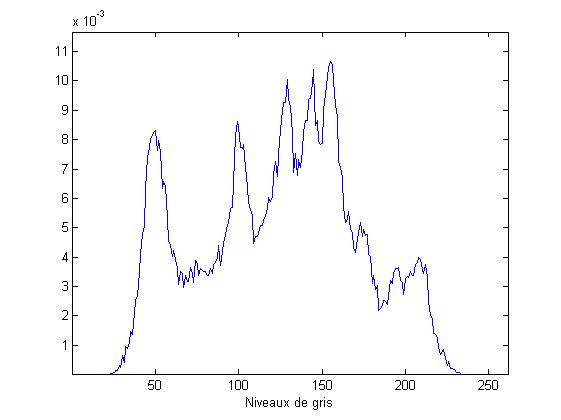
\includegraphics[scale=0.6]{../proba.jpg}
	 \caption{\label{probaGris} Distribution de probabilités, niveaux de gris}
\end{center}
\end{figure}




\section{Codeur arithmétique}

\section{Conclusion}


\clearpage
\appendix

\section{Codes source MATLAB}
\subsection{Algorithme - codage de Huffman}\label{algohuffman}

\FSource{../huffman.m}

\end{document}